%Feedback:
%A major challenge is how to simplify the gameplay so that starting the
%game is immediately a fun and funny experience. A core concept of the
%game is to parody a serious topic and use stereotypical things like
%praying and books in a humorous way. The gameplay should also support
%this effort, so that it is fun and funny, rather than serious and
%difficult. I would consider how to make the game work with only one or
%two players by including some simple AI concepts that fit this
%framework. For example, many AI players can be forming groups and
%casting wonders, but without much smarts or effectiveness. It's up to
%the human players to focus the efforts of the group in a strategic
%way.
%=================
%Summarized:
% - instant fun
% - game should work with 1,2 players
% - AI required

{\documentclass[11pt,a4paper,titlepage,table]{article}
\usepackage[a4paper]{geometry}
\usepackage[utf8]{inputenc}
\usepackage[english]{babel}
\usepackage{lipsum}



\usepackage{amsmath, amssymb, amsfonts, amsthm, fouriernc}
% mathtools for: Aboxed (put box on last equation in align envirenment)
\usepackage{microtype} %improves the spacing between words and letters

\usepackage{graphicx}
\graphicspath{ {./pics/} {./eps/}}
\usepackage{epsfig}
\usepackage{epstopdf}
\usepackage{colortbl}


%%%%%%%%%%%%%%%%%%%%%%%%%%%%%%%%%%%%%%%%%%%%%%%%%%
%% COLOR DEFINITIONS
%%%%%%%%%%%%%%%%%%%%%%%%%%%%%%%%%%%%%%%%%%%%%%%%%% 
\usepackage{colortbl}
\usepackage[usenames,dvipsnames,svgnames,table]{xcolor}
\usepackage{float}
%%%%%%%%%%%%%%%%%%%%%%%%%%%%%%%%%%%%%%%%%%%%%%%%%%
\definecolor{MyColor1}{HTML}{75A42E}
\definecolor{MyColor2}{HTML}{75A42E}
\definecolor{MyColor3}{HTML}{4D6D1E}
\definecolor{green1}{HTML}{EAF5DB}
\definecolor{green2}{HTML}{C2E193}
\definecolor{maroon}{cmyk}{0,0.87,0.68,0.32}
\newcommand{\textb}{\color{Black} \usefont{OT1}{lmss}{m}{n}}
\newcommand{\blue}{\color{MyColor1} \usefont{OT1}{lmss}{m}{n}}
\newcommand{\blueb}{\color{MyColor1} \usefont{OT1}{lmss}{b}{n}}
\newcommand{\red}{\color{LightCoral} \usefont{OT1}{lmss}{m}{n}}
\newcommand{\green}{\color{Turquoise} \usefont{OT1}{lmss}{m}{n}}
%%%%%%%%%%%%%%%%%%%%%%%%%%%%%%%%%%%%%%%%%%%%%%%%%%




%%%%%%%%%%%%%%%%%%%%%%%%%%%%%%%%%%%%%%%%%%%%%%%%%%
%% FONTS AND COLORS
%%%%%%%%%%%%%%%%%%%%%%%%%%%%%%%%%%%%%%%%%%%%%%%%%%
%    SECTIONS
%%%%%%%%%%%%%%%%%%%%%%%%%%%%%%%%%%%%%%%%%%%%%%%%%%
\usepackage{titlesec}
\usepackage{sectsty}
%%%%%%%%%%%%%%%%%%%%%%%%
%set section/subsections HEADINGS font and color
\sectionfont{\color{MyColor1}}  % sets colour of sections
\subsectionfont{\color{MyColor2}}  % sets colour of sections
\subsubsectionfont{\color{MyColor3}}  % sets colour of sections


%set section enumerator to arabic number (see footnotes markings alternatives)
\renewcommand\thesection{\arabic{section}.} %define sections numbering
\renewcommand\thesubsection{\thesection\arabic{subsection}} %subsec.num.

%define new section style
\newcommand{\mysection}{
	\titleformat{\section} [runin] {\usefont{OT1}{lmss}{b}{n}\color{MyColor1}} 
	{\thesection} {3pt} {} } 

%%%%%%%%%%%%%%%%%%%%%%%%%%%%%%%%%%%%%%%%%%%%%%%%%%
%		CAPTIONS
%%%%%%%%%%%%%%%%%%%%%%%%%%%%%%%%%%%%%%%%%%%%%%%%%%
\usepackage{caption}
\usepackage{subcaption}
%%%%%%%%%%%%%%%%%%%%%%%%
\captionsetup[figure]{labelfont={color=MyColor1}}


\makeatletter
\let\reftagform@=\tagform@
\def\tagform@#1{\maketag@@@{(\ignorespaces\textcolor{red}{#1}\unskip\@@italiccorr)}}
\renewcommand{\eqref}[1]{\textup{\reftagform@{\ref{#1}}}}
\makeatother
\usepackage{hyperref}
\hypersetup{colorlinks=true}

%%%%%%%%%%%%%%%%%%%%%%%%%%%%%%%%%%%%%%%%%%%%%%%%%%
%% PREPARE TITLE
%%%%%%%%%%%%%%%%%%%%%%%%%%%%%%%%%%%%%%%%%%%%%%%%%%
\title{\blue  
	\begin{figure}[h!]
  		\centering
    	\includegraphics[width=1\textwidth]{img/logo3}
	\end{figure}
	\blueb Battle of Origins | Paper Prototype}
\author{Patrick Misteli, Ruben Kälin, Jacqueline Staub, Gregory Wyss}
\date{\today}
%%%%%%%%%%%%%%%%%%%%%%%%%%%%%%%%%%%%%%%%%%%%%%%%%%



\begin{document}
	\maketitle
	\hypersetup{linkcolor=MyColor1}	
	
	\tableofcontents
	\newpage
	
	\section{Introduction}
	During the creation of the paper prototype our focus was on the following core features of our game:\\
	
	\begin{itemize}
		\item Evolution of attack, speed and praying/studying-capabilities of every player
		\item Creating big wonders and converting players from the opposing team
		\item Suitable behaviours of the artificial intelligence controlling NPCs
		\item A map with obstacles, allowing players to hide, and search for good paths
	\end{itemize}
	
	In the following chapter we present the individual components of our board game. Chapter \ref{rules} elaborates our set of rules as well as the process of finding suitable rules (that can be adapted for the real game). We state the challenges we encountered during the making of the prototype in Chapter \ref{findings} and conclude by explaining the most influential findings. 
		
	\section{Creating the prototype}
	\label{sec:creatingPrototype}
	Using cardboard, paper, scissors and glue we assembled a board game for up to 8 players (controlled by a human or by a simulation of an artificial intelligence, whose behaviour we fixed before the game). In the most primitive version, the artificial intelligence only determines the closest player, walks towards him and depending on its team membership tries to study/pray with him or attempts to shoot him.
	
	\subsection{Player tokens}
	
	All tokens either belong to the group of \textit{religionists} or the group of \textit{scientists}. They can be distinguished by comparing the item on their head. The token belongs to the religionists if the item on it's head is a \textit{halo}. Otherwise (if it is a \textit{university hat}) it belongs to the scientists, see Figure \ref{fig_tokens}.
	
	\begin{figure}[h!]
  		\centering
    	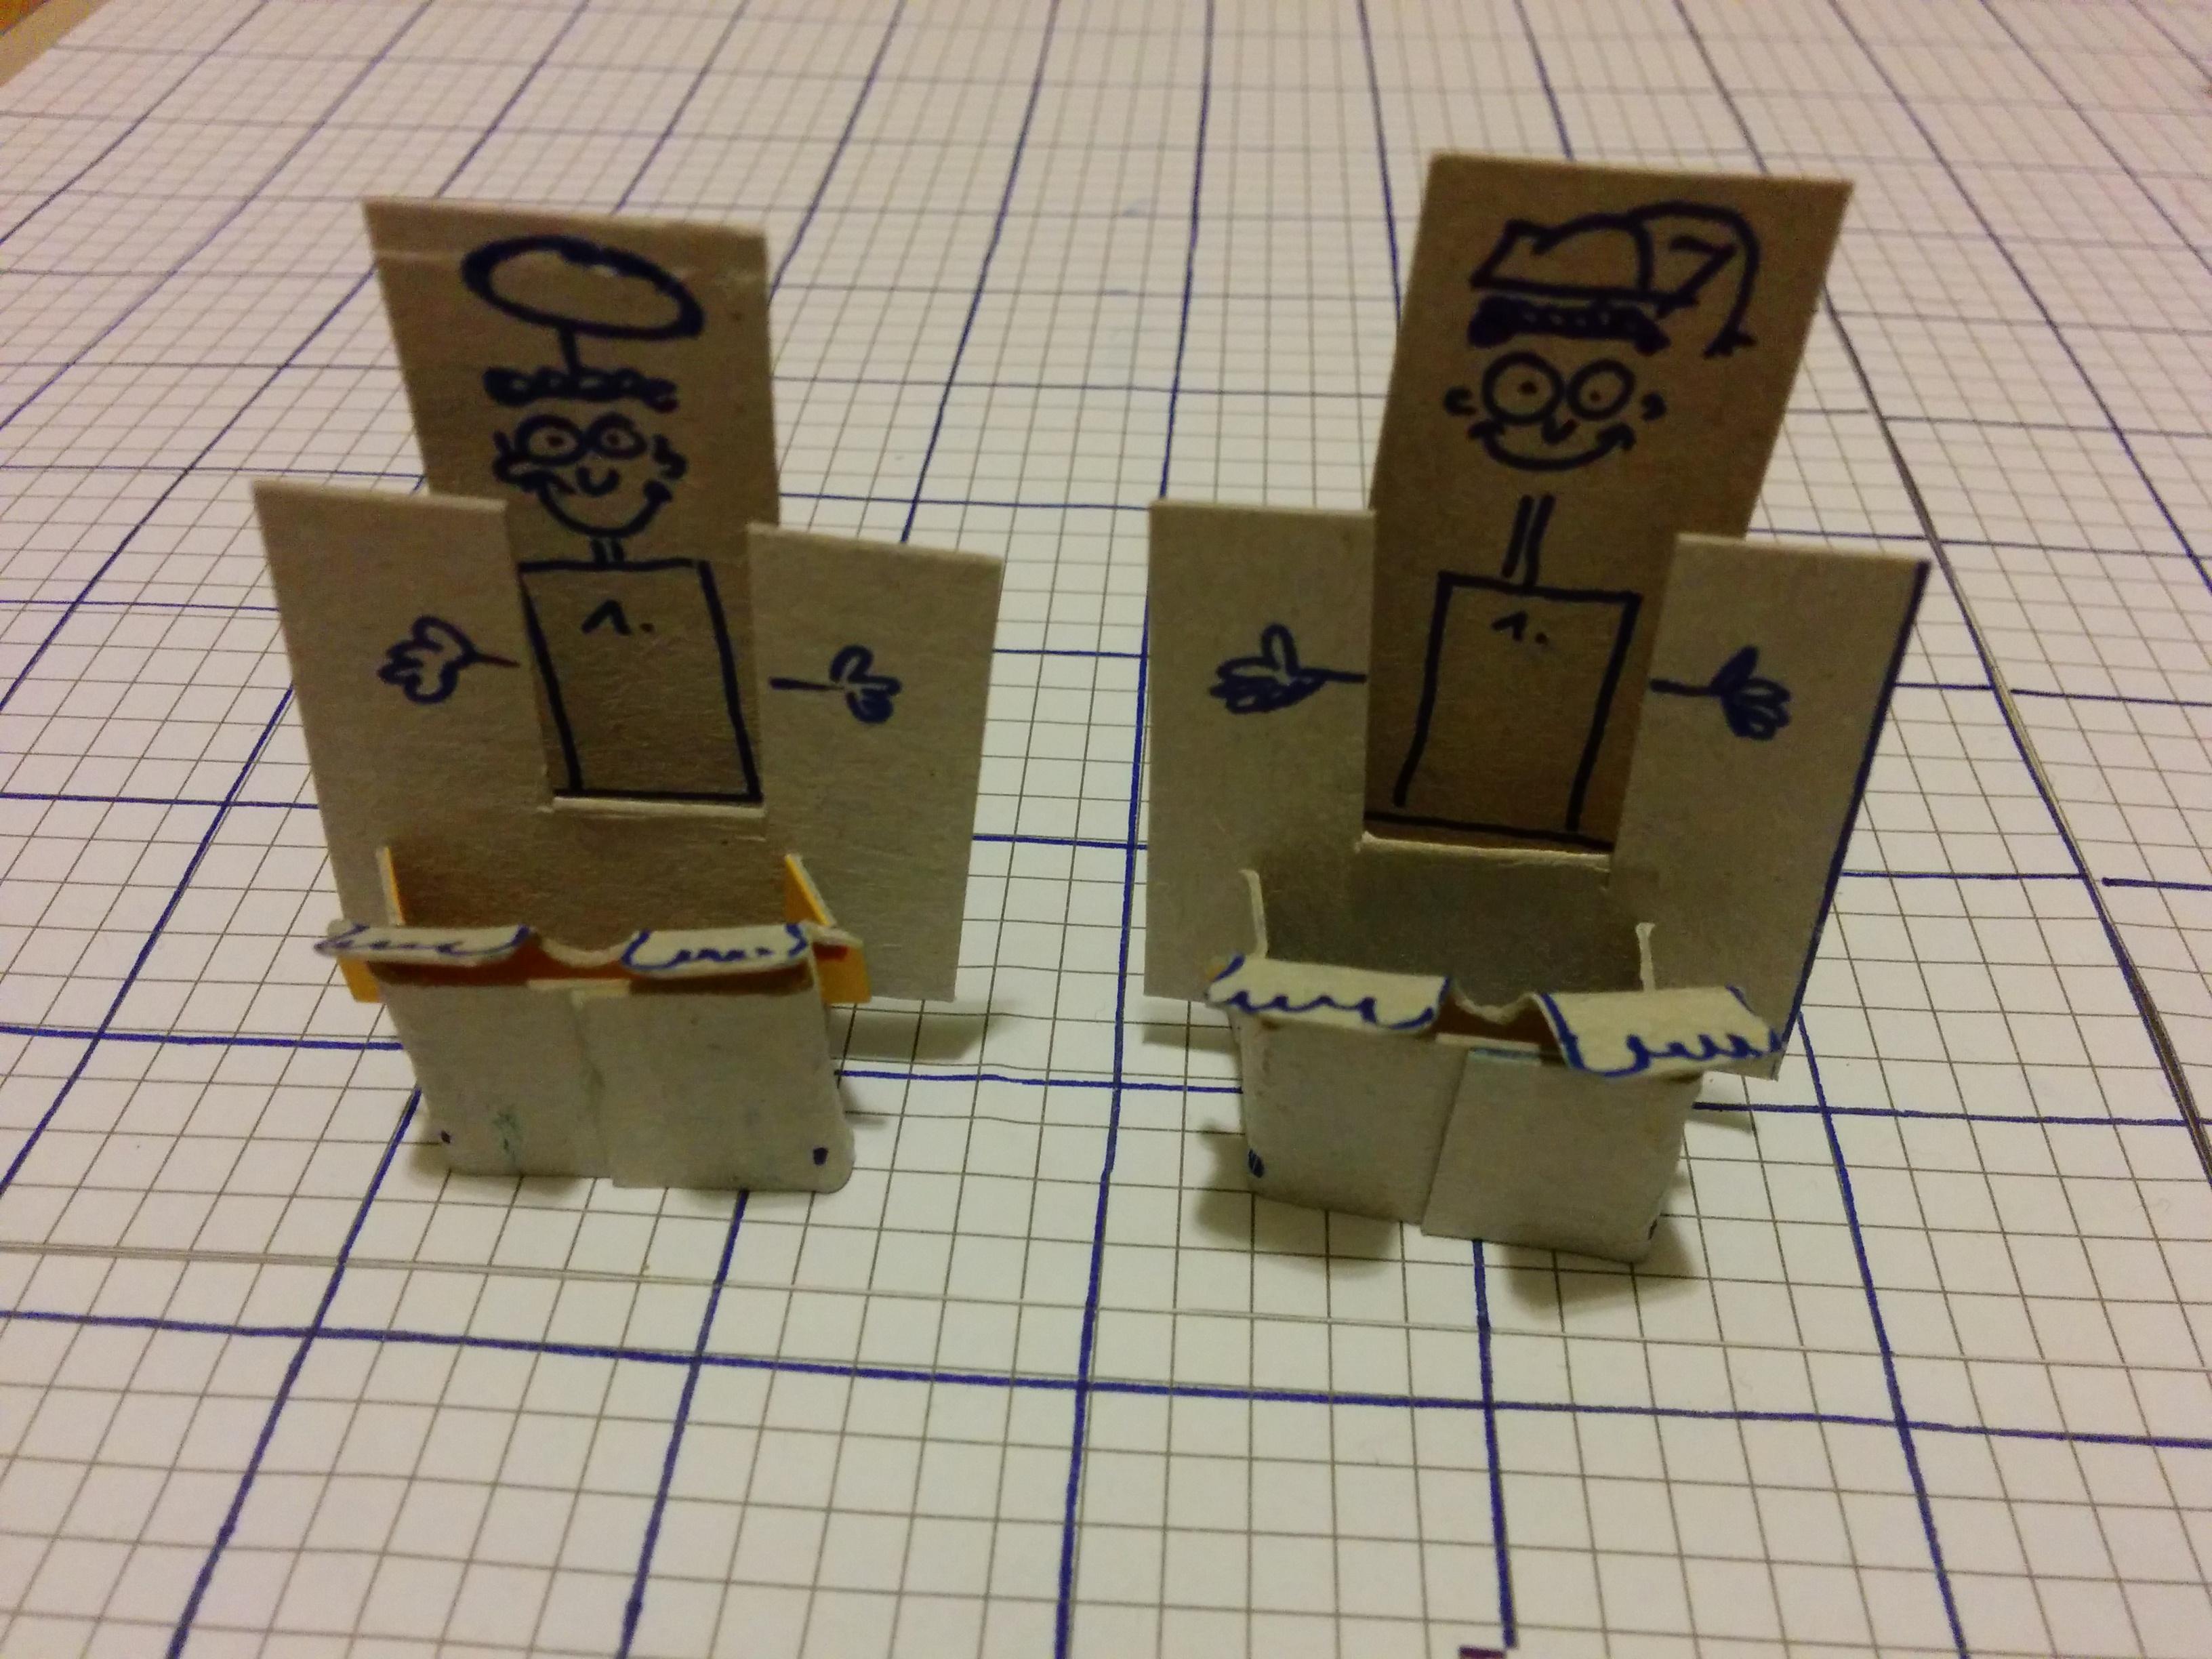
\includegraphics[width=0.7\textwidth]{img/tokens}
    	\caption{religionist token (left) and scientist token (right)}
    	\label{fig_tokens}
	\end{figure}
	
	Every token has a little number on its back in order to tell multiple tokens of the same group apart. Every player is assigned to one token, from that moment on he fights with the according token until he gets converted, which is when he is assigned another token of the same group, if there is one left, which is not played by a human player.\\
	
	\subsection{Obstacles}
	
	We introduced walls in our board game to allow the players to hide from their opponents, see Figure \ref{fig_board}. The walls urge the players to find a strategic position that is hard for an opponent player to reach or from which it is easy to escape a dangerous situation.
	
	\begin{figure}[h!]
  		\centering
    	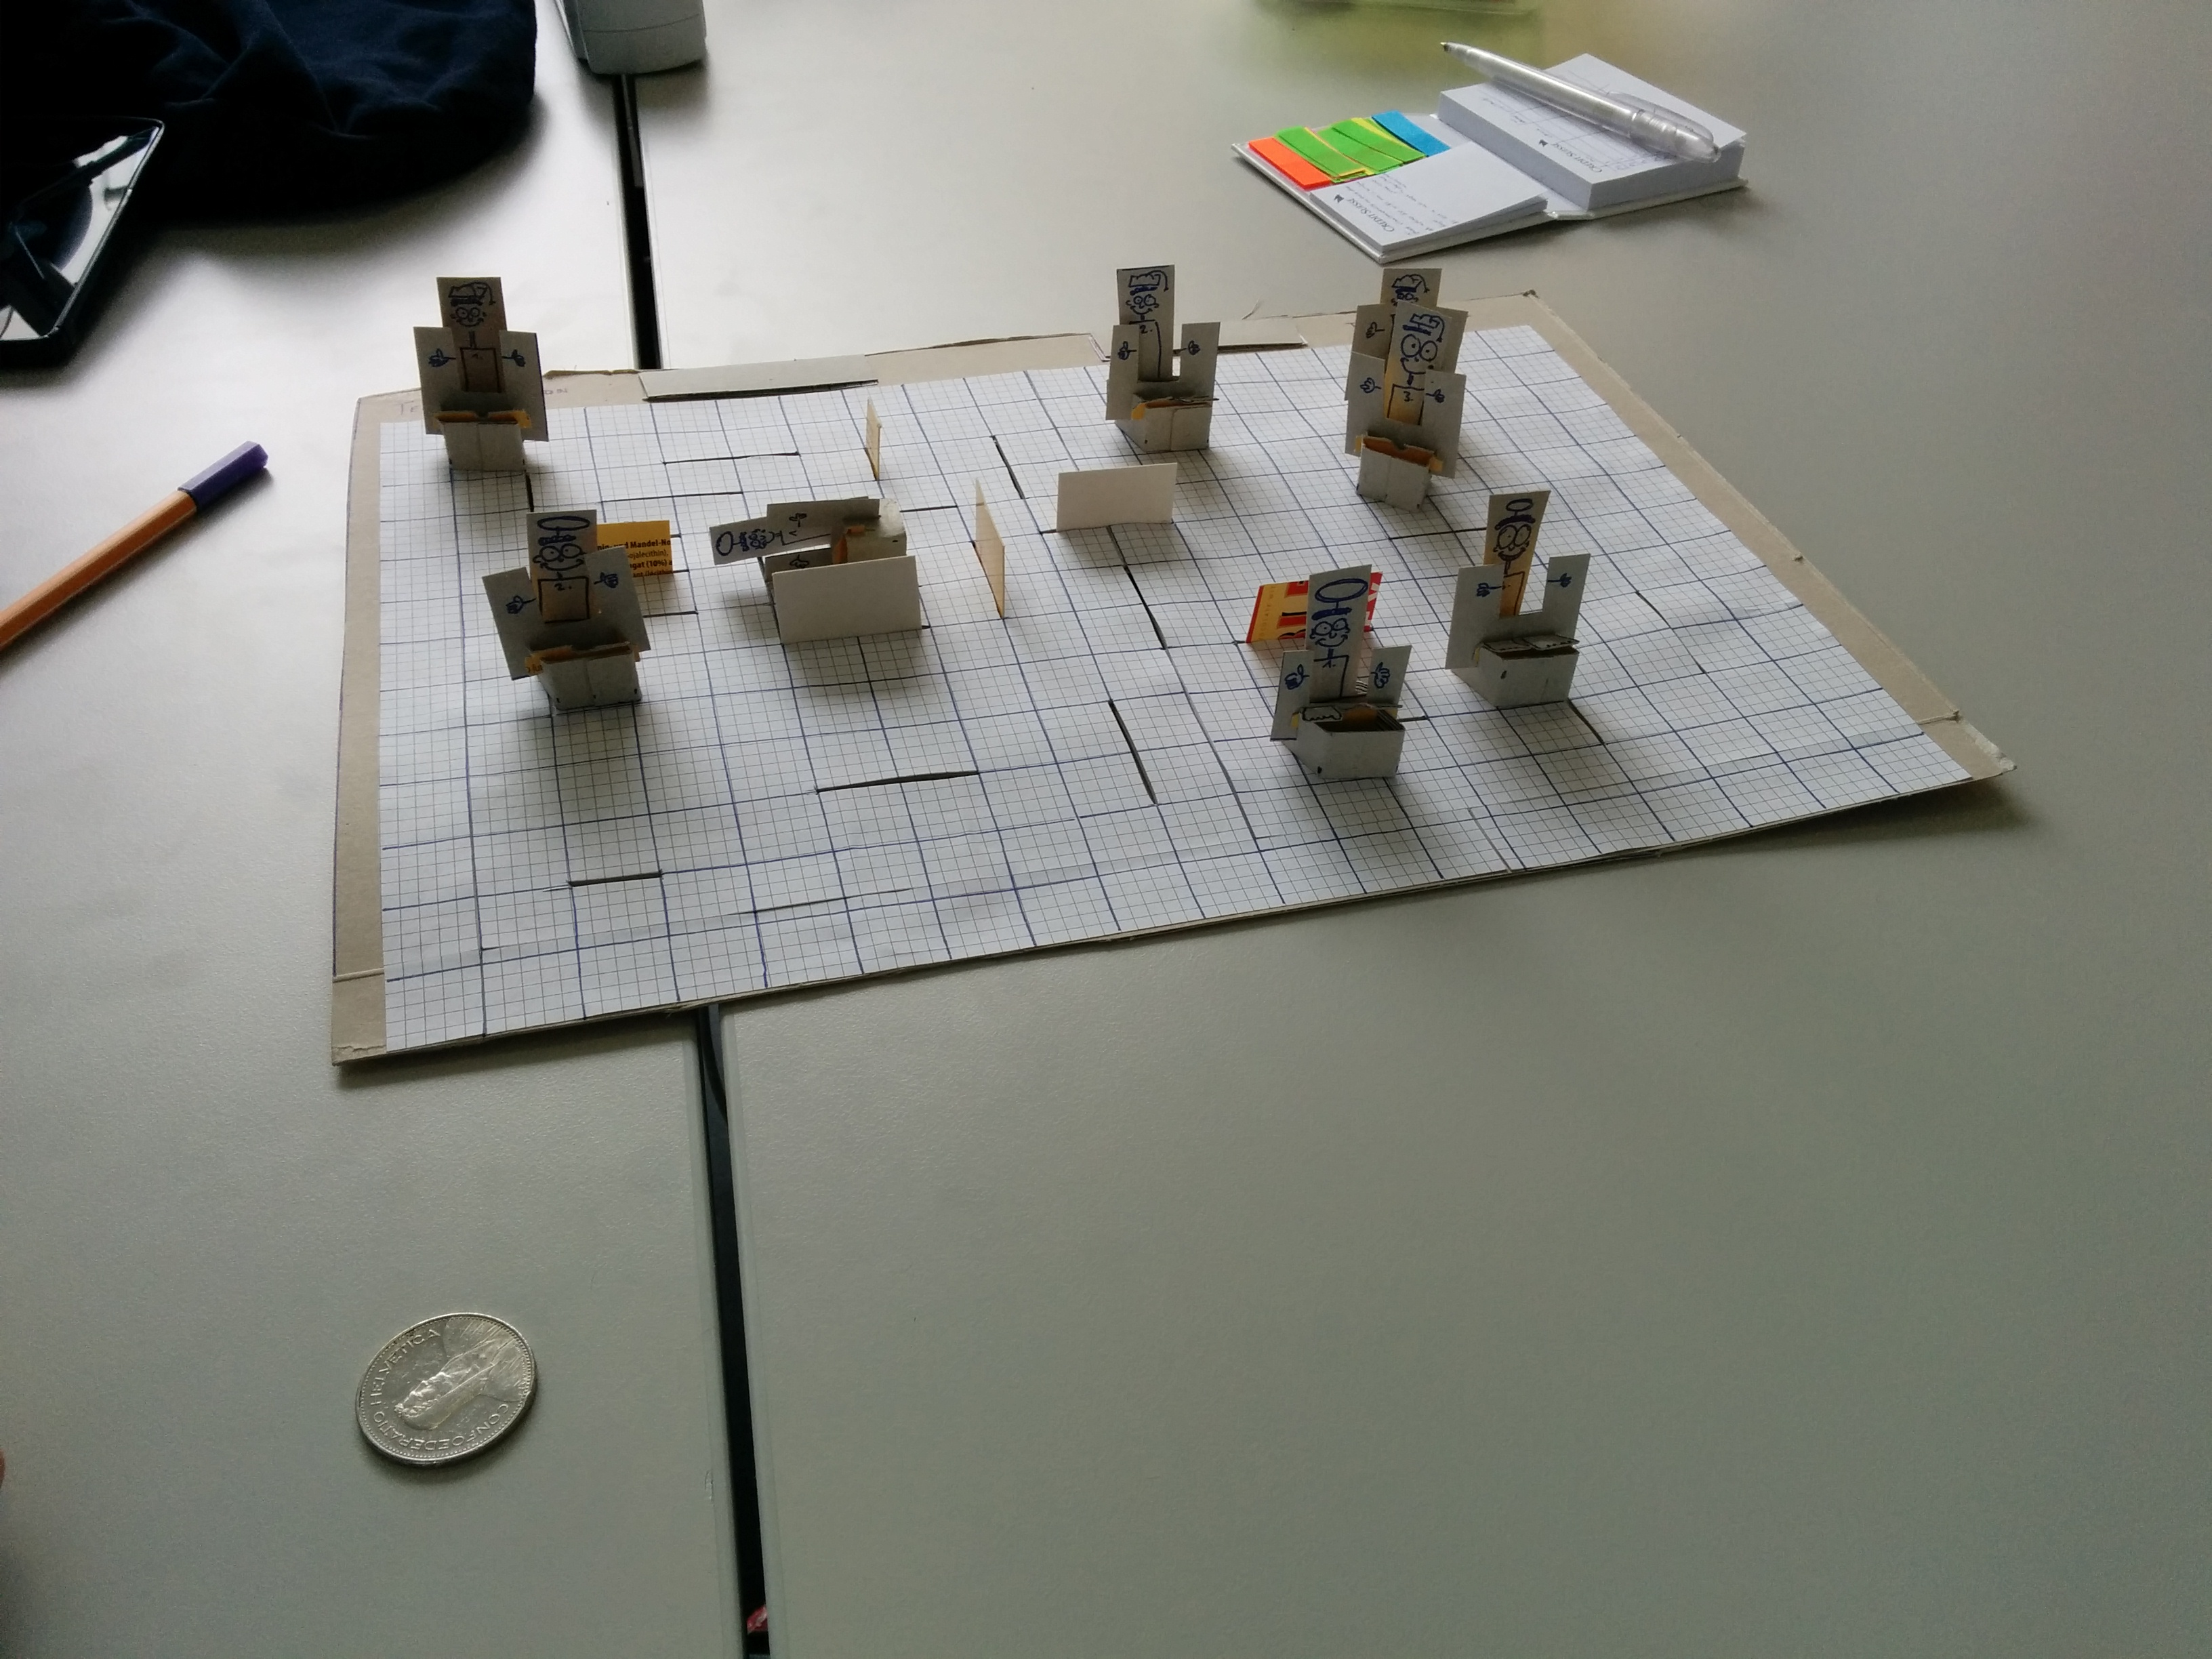
\includegraphics[width=0.7\textwidth]{img/prot3}
    	\caption{The board with walls as obstacles}
    	\label{fig_board}
	\end{figure}
	
	We wrote down our findings concerning the positioning of the walls and the possible impact of having corners in Chapter \ref{findings}.
	
	\subsection{Big wonder}
	
	Two or more people can get together to pray (if they are religionists) or study (if they are scientists). The more people gathered and the more evolved the people in a group are, in respect to praying/studying, the faster they can fill the progress bar. Once the progress bar on top of the board reaches the end, a big wonder for the corresponding group can be evoked. In the board game this is represented by an orange sticker, which is put on top of a randomly chosen player of the group holding the wonder. He can then walk around and try to convince as many enemies of his belief as possible (by just getting close to them). The player profits from an increased speed while the possessing a big wonder.
	
	\subsection{Interaction of players}
	
	In the real game every player has a controller and can walk around, turn and shoot as fast as he can press the corresponding buttons or move the joystick around. In our board game we had to make sure that every player gets a fair chance to do his turn at the same time as everybody else. Therefore we decided on a round-based board game using the following 8 types of actions:
	\begin{itemize}
		\item \textbf{Move in all directions:} $\uparrow$   $\leftarrow$  $\downarrow$  and $\rightarrow$
		\item \textbf{Attack}
		\item \textbf{Pray/Study}
	\end{itemize}
	
	Every player can move his token around, attack other players or get together with other players to pray or study. Each player has a set of 8 cards (one for each possible action). A subset of these can been seen in Figure \ref{fig_cards}. In one turn all human players put down one card before the computer performs the corresponding action for every other player. Once each player has committed to an action for this turn, all the actions are executed. This strategy enables a fair real-time game play experience while still being playable on a board.
	
	\begin{figure}[h!]
  		\centering
    	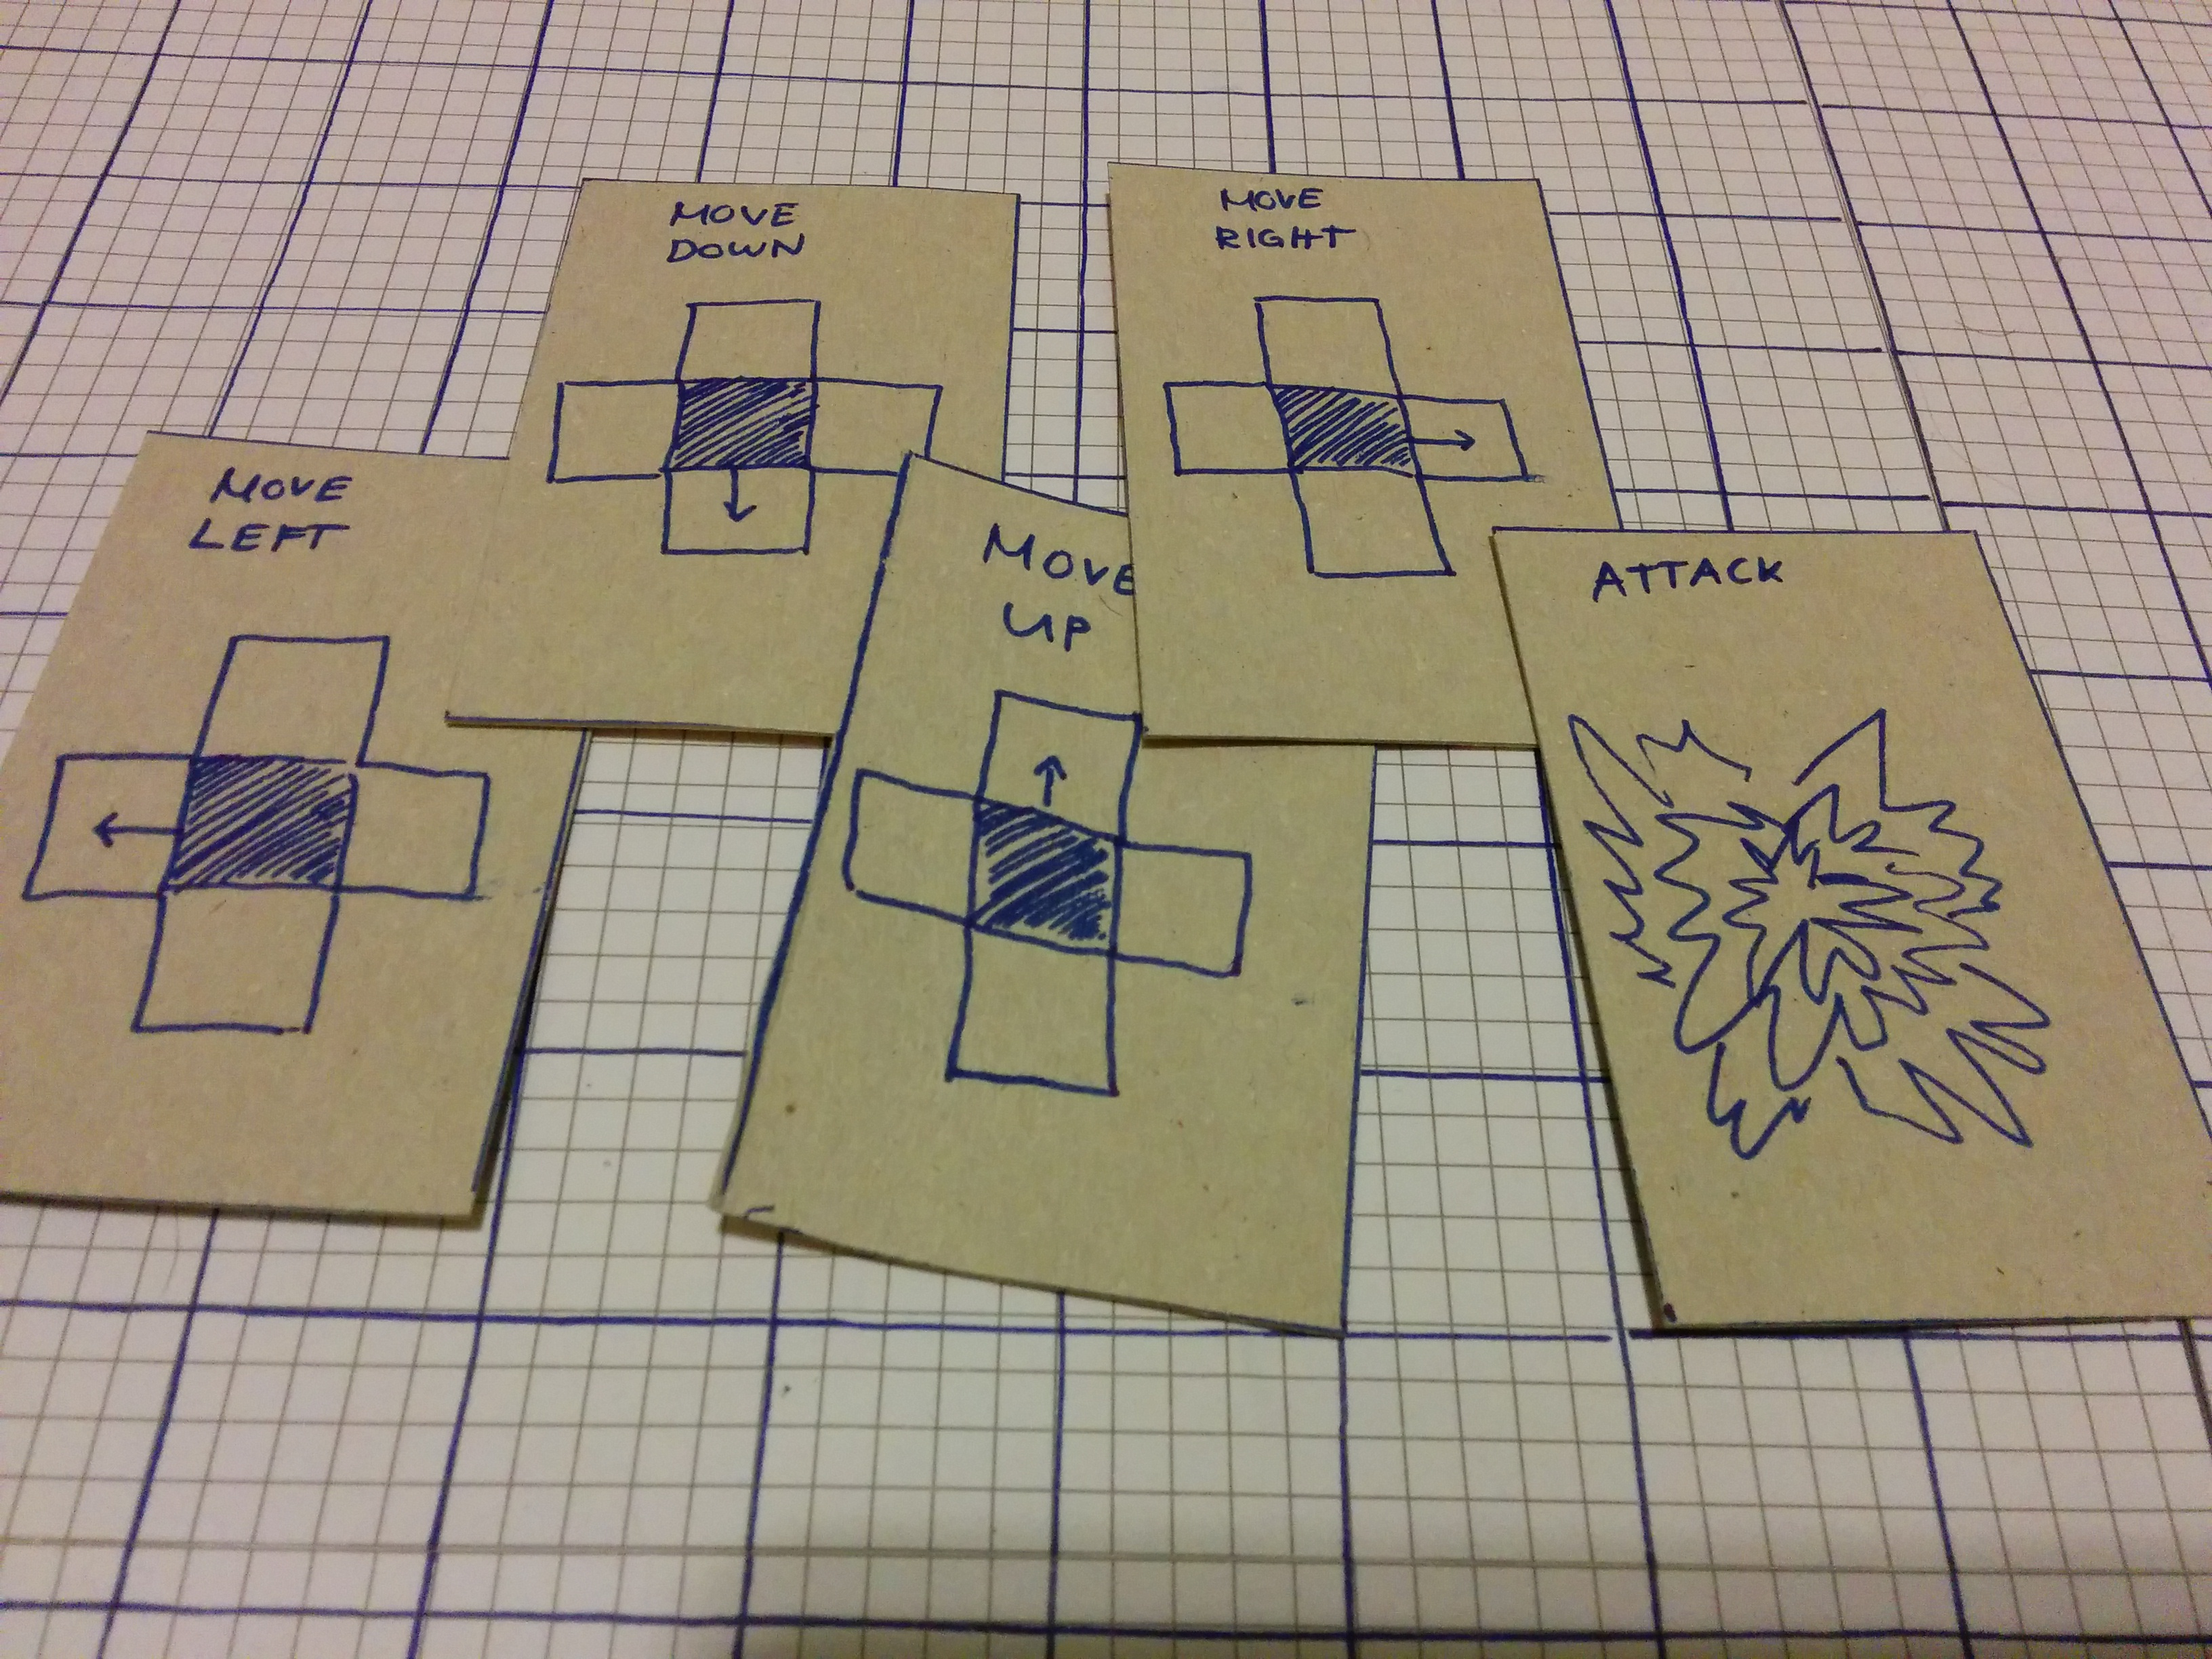
\includegraphics[width=0.7\textwidth]{img/cards}
    	\caption{cards, used in round-based board game}
    	\label{fig_cards}
	\end{figure}

	\section{Gameplay/Rules}\label{rules}
	
	In this section we will discuss the rules proposed for the board game.
	
	\subsection{Preparation}
	
	\begin{enumerate}
		\item Every player chooses one side, either becoming “scientist” or “religionist”. Add as many additional playing pieces as desired but making sure to end up with two equally large teams. Every player gets…
		\begin{itemize}
			\item[a)] the following set of playing pieces, containing:
			\begin{itemize}
				\item[i.] 1 socket
				\item[ii.] 1 pair of feet
				\item[iii.] 1 pair of hands
				\item[iv.] 1 torso with head
			\end{itemize}
			\textit{These pieces should be plugged together.}
			\item[b)] a set of cards, containing:
			\begin{itemize}
				\item[i.] 3 cards: move up
				\item[ii.] 3 cards: move down
				\item[iii.] 3 cards: move left
				\item[iv.] 3 cards: move right
				\item[v.] 1 card: attack
				\item[vi.] 1 card: pray/study
			\end{itemize}
			\textit{Every player has to take all of these cards into his hands and is not allowed to show them to the other players.}
			\item[c)] a set of 9 colored stickers, composed of:
			\begin{itemize}
				\item[i.] 3 green stickers
				\item[ii.] 3 yellow stickers
				\item[iii.] 3 red stickers
			\end{itemize}
			\textit{Every player is supposed to stick the three green stickers on his token's feet, head and hands. These are the visual representations of their current skill points. Feet = Running speed, Hands = Attack strength, Head = Praying/Studying contribution}
		\end{itemize}
		For each AI-controlled player the computer gets all the items.
		
		\item Take the board and put it on a table.
		\begin{itemize}
			\item[a.] There are 17 walls (either 1 or 2 units long). Plug some of them into the board, by pushing the walls from below through the slot of the board. Feel free to create your own playground. This modular design allows for a multitude of different levels using the same board.
			\item[b.] The board consists of 13*19 fields. To determine the starting position of the players each player throws two 20-sided until the first die is in the range 1 to 13 and the second is in the range 1 to 19. In case some other player is already at the determined location, the process is repeated, otherwise the token is placed there.
			\item[c.] In the upper region of the board you can see two progress bars. Cover them completely by using the two masking strips. Figure \ref{fig_firstPrototype} shows the first version of our board.
		\end{itemize}
		\item The notebook is held and administrated by the computer.
	\end{enumerate}
	
	\begin{figure}[h!]
  		\centering
    	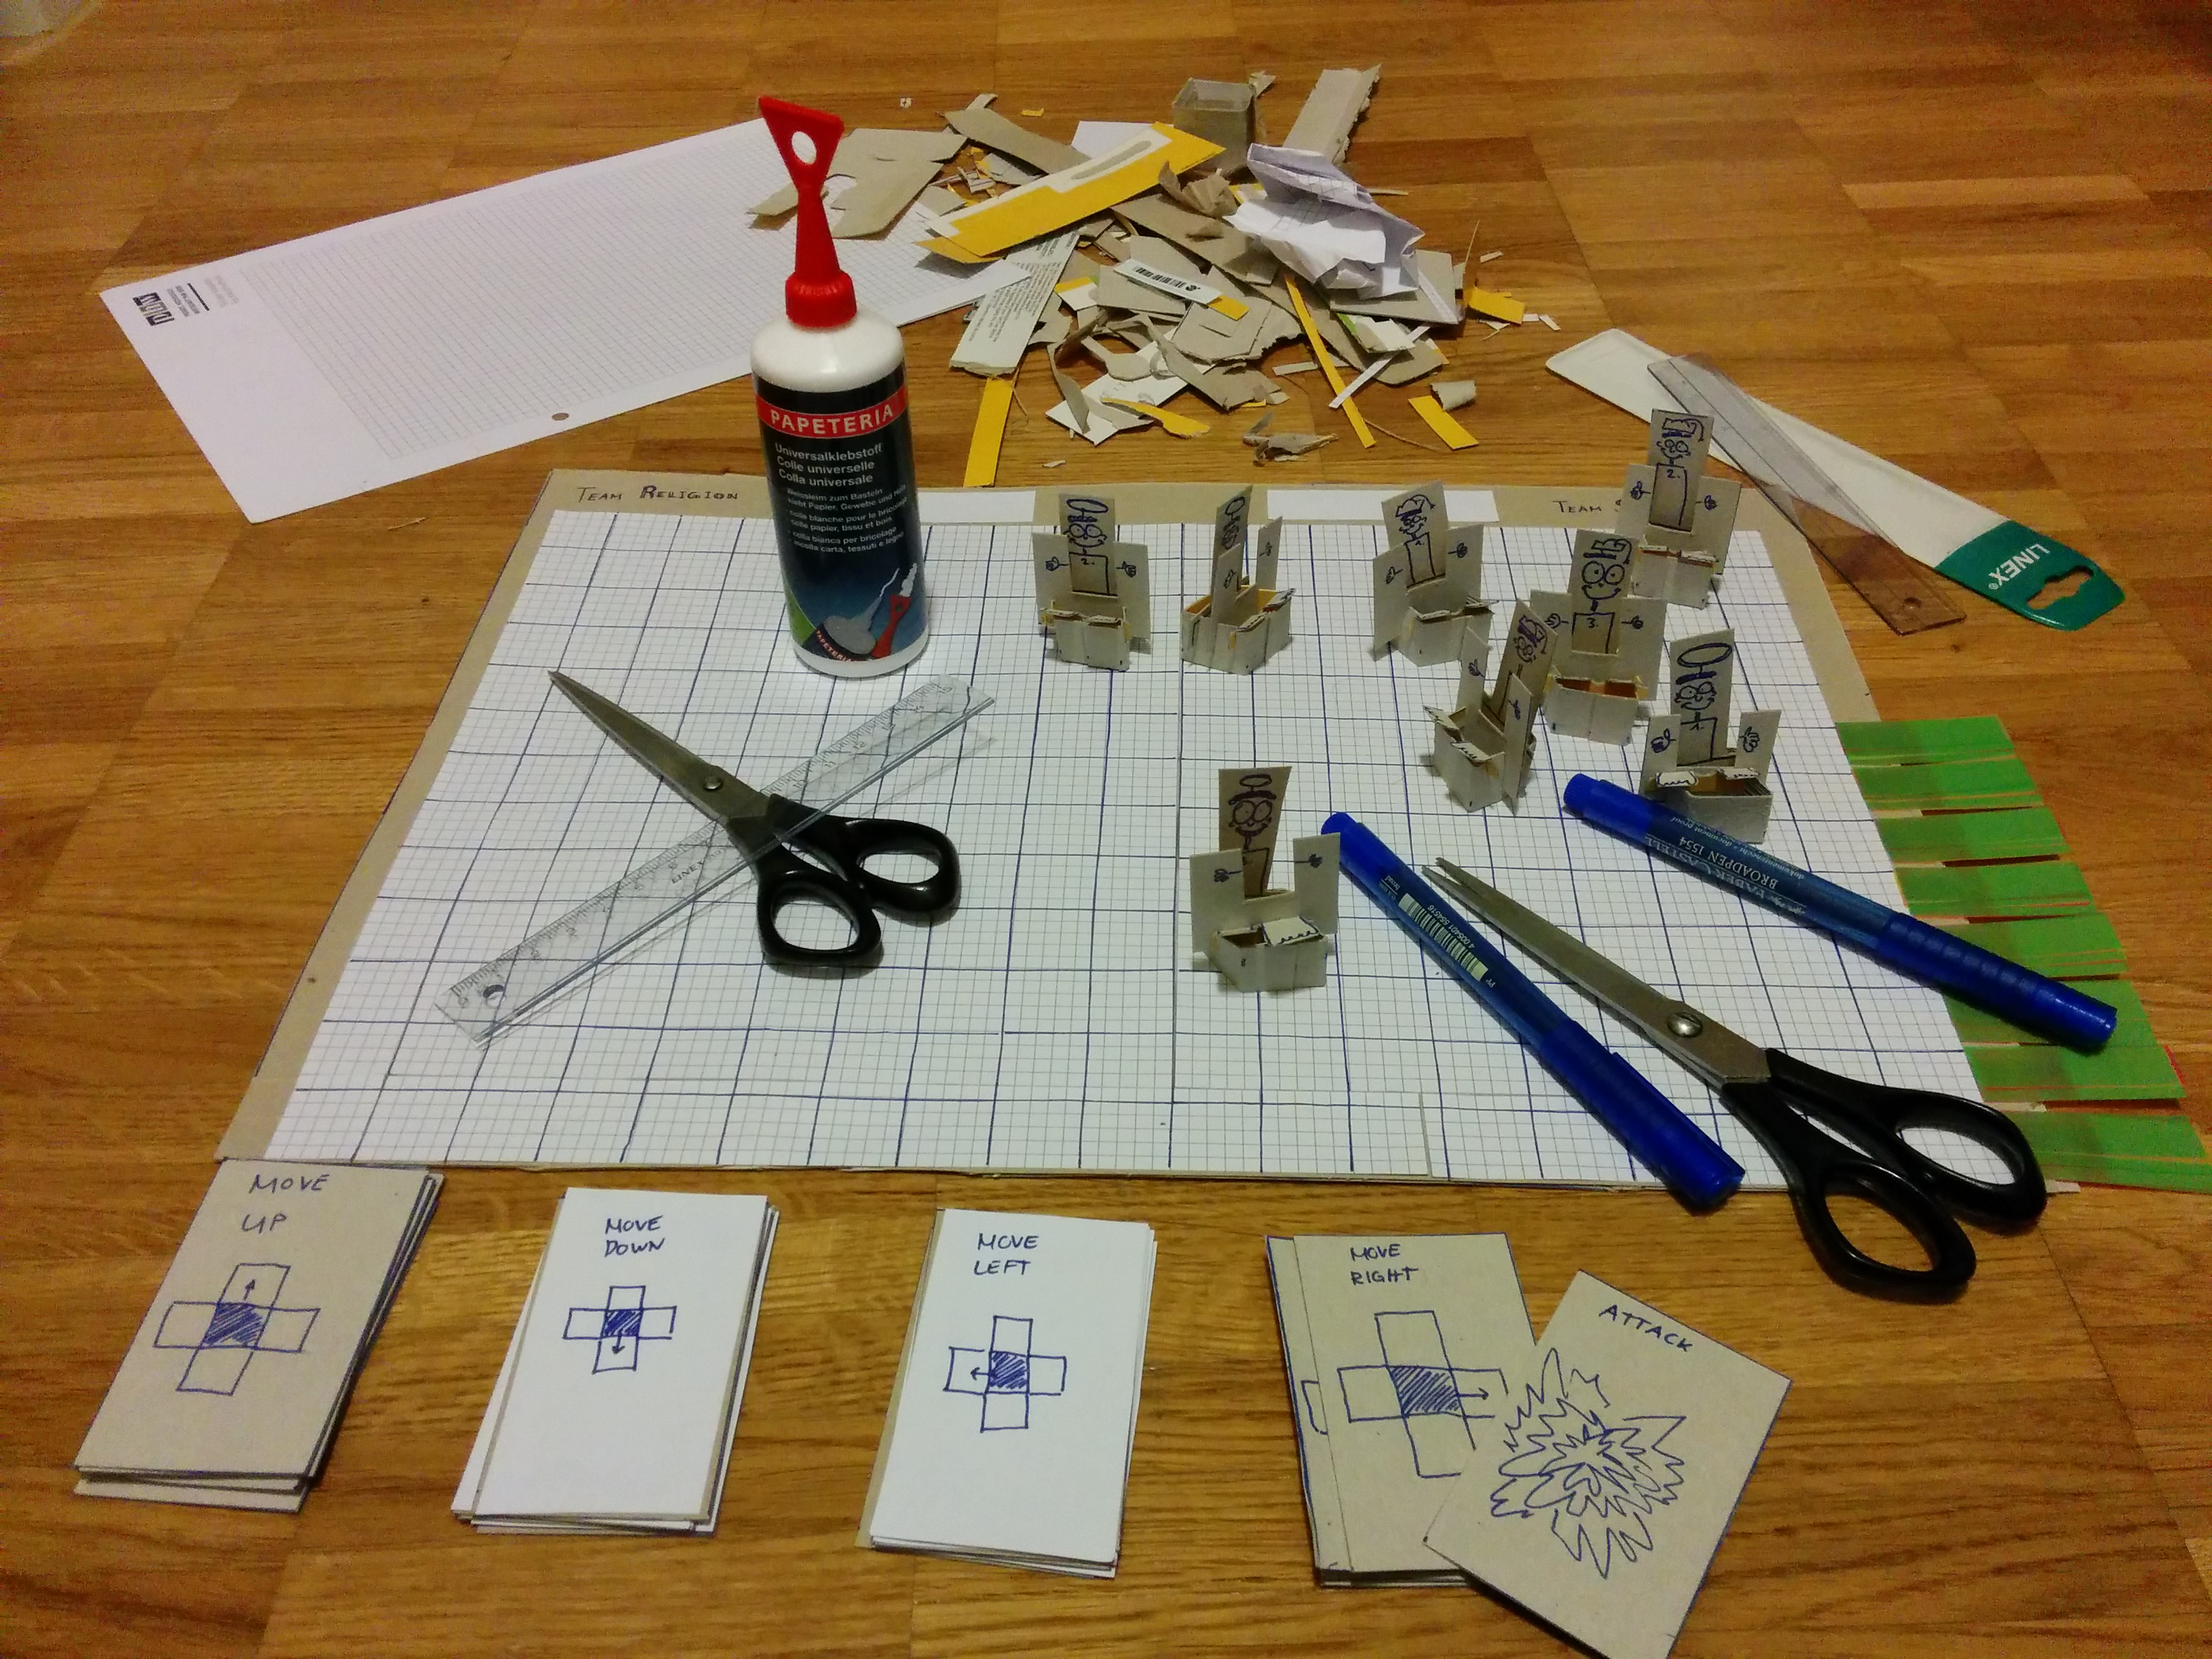
\includegraphics[width=0.7\textwidth]{img/prot1}
    	\caption{the first version of our board game (walls not attached yet)}
    	\label{fig_firstPrototype}
	\end{figure}
	
	\subsection{Goal}
	
	The goal of the game is to convince all the players of the opposite team of your belief.
	
	\subsection{Game principle}
	
	The game is performed round-wise. One round is based on two sessions: All the players put one of their cards facing down in front of them. Afterwards, the computer turns all the cards around and performs the actions. The players have the following options: In every round they can either move up, down, left or right, try to attack some other player with the attack card or pray/study (depending on the team membership). All of the actions get noted in the notebook. Whenever a player moves in a round, the computer keeps track of this in the notebook by putting a sign in the column “movement” on the according row of the player. For all the three activities (study/pray, attack and move) the players can upgrade from the green to the yellow sticker when they performed the action 10 times. Another upgrade from yellow to red kicks in after performing the action another 15 times. (Notice: The double/triple movement when having the yellow/red sticker still count only as 1 movement when notated in the notebook).
	
	\subsection{Movement}
	
	Whenever a player decides on a movement card this has an effect. The strength of the effect depends on the player's movement strength (the color of the sticker on his feet). Someone who has a green sticker on his feet can move exactly one field up, down, left or right per round. Someone with a yellow sticker can move up to two fields into the directions: \textit{UP}, \textit{DOWN}, \textit{LEFT} or \textit{RIGHT}. (They can be used repeatedly, so a movement left-left would be okay for someone with a yellow sticker). They indicate their movement by choosing the according cards and by putting them down in the according order. The uppermost card gets performed first. The same way someone with a red sticker on his feet can move up to 3 fields per round, indicating this by putting the according cards in the corresponding order.
	
	\subsection{Attack}
	
	The attack is directed. If some player plays the attack-card, all of the fields in front of the player are affected. Depending on the distance the effect is more serious. Every player of the opposite team who is standing in one of the affected fields gets pushed away and is not able to move or attack or study/pray. The duration of the stunning depends on the attack strength (sticker color of the hands of the attacker) and distance of the attack. If the attacker has a green sticker on his hands, the victim gets thrown away 2 fields and is stunned for 2 rounds. If the attacker has a yellow sticker, the victim gets thrown away 3 fields and is stunned for 3 rounds. And if the attacker has a red sticker, the victim gets thrown away 4 fields and is stunned for 4 rounds. All of these numbers are calculated for attacks which are fired very close (just one field away). If the attack gets fired from farther away, the effect decreases by the distance. (Note: In the real game we will make the amount of time a player gets stunned dependent on his defence strength as well as on the attack strength and the distance.)
	
	\subsection{Study/Pray}
	
	The study/pray card only has an effect if some players are standing close (on one of the 8 neighbouring fields) and if they decided on studying or praying as well. The effect of the studying/praying is, that the team’s progress bar on top of the board gets filled up. Every player with a green head-sticker contributes 1 field of the power-strip to be filled in every round he is studying/praying. Every player with a yellow head-sticker contributes 2 study/pray-units. And every player with a red head sticker contributes with 3 study/pray-units. Once the power strip is full, one of the players of the according team is chosen randomly (using a 6-sided dice), who gets the big wonder. A player with a big wonder can move around and will convert everybody standing close to him (on one of the neighbouring 8 fields). The big wonder keeps going for 5 rounds. If a group decides to disperse, the progress bar stays as it was until a new group meets to pray or study. If a human player gets converted, his token gets converted and the human player takes control of a token, which was not controlled by a human before.
	
	\section{Findings}
	\label{findings}
			\subsection{Map Design}	
				The map should not include any corners where players can stand together. When being shot they will simply be hurled further into the corner, thus making splitting up a praying/studying group impossible. This must be taken into consideration when adding obstacles to the map. The problem remains with the edges and corners of the frame of the map. We solve this by making the map continuous. I.e. a player can walk "out" on the left side of the map and will reappear on the right side.
				
			\subsection{Wonder Possession}
				Possessing the wonder gives a temporary increase of speed to the player to make the game more interesting. He will then have a higher chance of converting an opponent. 
				Furthermore while the wonder is active he is immune to all type of attacks (main attacks and conversions). This prevents a player from being converted while currently converting others leaving him as a more powerful player.

			\subsection{Conversion of Human Player}
				Once a player is converted he takes over a NPC from the same team.
			\subsubsection{Hit Cooldown}
				Once a player is hit he has a cooldown period where he is not able to attack. In the real game this will be visually represented by the character getting on his feet again.
			
			\subsubsection{Immunity Cooldown}
				Once a player is on his feet again he is immune to main attacks for a while. This prevents a player firing at another player and waiting until he is back on his feet to immediately shoot him again. 
				
			\subsubsection{Committing to wonder creation}
			\label{subsubsec:commit_to_wonder}
				We realized that it was possible to study/pray, wait for the opponent to arrive, shoot him away and continue studying. This was a very easy winning strategy and decreased the overall fun of the game. We therefore introduced a commitment to the wonder creation. Once standing together you can commit to the wonder creation. During this time your immunity is very high (meaning you will be hurled further away) and cannot attack. In addition there is a cooldown period. Once you stopped committing to praying/studying you need to wait 1 turn (a few seconds in the real game) before being able to shoot again.
				
			\subsubsection{Shot Impact}
				The distance being hurled away and the cooldown until a player is back on his feet again depends on the following factors:
				\begin{itemize}
					\item \textbf{Distance between shooter and target}
					\\small distance = more damage
					\\large distance = less damage
					\item \textbf{Accuracy of shot} \\
						Being hit directly = more damage
						\\Not standing exactly in the direction of the shot, but still in the spread = less damage
					\item \textbf{Attack skill of Shooter}
						\\higher skill = more damage
					\item \textbf{Defence skill of target}
						\\higher skill = less damage
				\end{itemize}
				
			\subsubsection{AI}
				The AI can be simplified at the beginning as proposed and described in Chapter \ref{sec:creatingPrototype}. More complex AI might take into account whether currently other study/praying groups exist. Merging two small studying/praying groups into one yields a speed up in the wonder creating process.
				
			\subsection{Timelimit}
				Instead of waiting for a team to convert the other completely a limit of round numbers can be added. This ensures a quick gameplay. In the real game a time limit in minutes can be added. The winner of the game is the team with the most members when the time runs out.
				
				\subsection{Strategies}
				An important factor for balancing the gameplay are the strategies and their effectiveness. During playing the board game we encountered three different main strategies. First, a player can move as fast as possible towards an opponent and try to restrain the enemy of praying/studying by shooting them away. Players using this strategy are called \textit{destroyer}. Second, a less aggressive strategy is to move towards team members and to start praying/studying as soon as possible so that the big wonder bar is filled quickly. We call players using this strategy \textit{converter}. Third, a hybrid of strategy one and two allows a player to study when the opponent is far away, but also to defend himself if the enemy is coming to blow up your praying/studying circle. Players using this strategy are named \textit{hybrids}.				
				\\
				As one can imagine a team needs both \textit{destroyer} and \textit{converter}. Without \textit{destroyer} the enemy can fill its big wonder bar very fast and start to convert you after a short amount of time. On the other hand, without \textit{converter} a team will have severe issues to cast a big wonder and therefore cannot win the game. Nevertheless, during playing the board game the \textit{hybrid} strategy was not as effective as the other two patterns due to the fact that the specific skills are evolving much faster for the \textit{converter} and \textit{destroyer} because they focus on doing one thing. In addition a \textit{hybrid} requires good timing since we introduced a cool-down after praying/studying before being able to shoot again (shown in section \ref{subsubsec:commit_to_wonder}). Additionally, during the cool-down period the player cannot practice its skills. Thus, switching between offensive and defensive strategies too often is discouraged.
				\\
				In our computer game we have to be careful how we evolve the skills of the characters so that none of the strategies has an advantage over the others. Also, we want to have the \textit{hybrid} strategy as an attractive way to play the game and we need to try out how the evolving curves will have to be applied. We like very much that different strategies need to be included in one team because we think that team spirit significantly increases the long-time fun factor since there is a lot to experiment with.
		
		\newpage			
		

\end{document}}{den}
